%% CLASS MANUAL FOUND IN http://blog.poormansmath.net/latex-class-for-lecture-notes/ %%
%% CLASS AUTHOR Stefano Maggiolo %%
\documentclass[english,course]{Notes}

\title{2B : Linear Algebra}
\subject{Mathematics}
\author{Joao Almeida-Domingues}
\email{2334590D@student.gla.ac.uk}
\speaker{Dr. Chris Athorne}
\date{23}{09}{2019}
\dateend{04}{12}{2019}
\place{University of Glasgow}

 %%%%% GENERAL MATHEMATICAL NOTATION SHORTCUTS %%%%%
 
\newcommand{\n}{\mathbb{N}}
\newcommand{\z}{\mathbb{Z}}
\newcommand{\q}{\mathbb{Q}}
\newcommand{\cx}{\mathbb{C}}
\newcommand{\real}{\mathbb{R}}
\newcommand{\field}{\mathbb{F}}
\newcommand{\ita}[1]{\textit{#1}}
\newcommand{\oneton}{\{1,2,3,...,n\}}
\newcommand\ef{\ita{f} }

\newcommand\inv[1]{#1^{-1}}
\newcommand\setb[1]{\{#1\}}
\newcommand\en{\ita{n }}
\renewcommand\qedsymbol{QED} %QED instead of square
\newcommand\handleft{\HandCuffLeft}
\newcommand\handright{\HandCuffRight}

%MATRICES
\usepackage{todo,float}
\usepackage[delims={[]}]{spalign}
\let\mat=\spalignmat
\let\amat=\spalignaugmat
\let\vec=\spalignvector

%%%%%%%%%%OPERATORS



%%%%%%%%%%%%%%%%%%
% row ops
\newcommand\ro[2]{\xrightarrow[#2]{#1}}

\setlength\parindent{0pt}
%%%%%%%%%%%%%%%%PACKAGES%%%%%%%%%%%%%%%%%%%%%%%%%%%%%
%\usepackage{lipsum}  

\usepackage{amsmath,amsthm,amssymb,graphicx,mathtools,tikz} %maths
\usepackage{hyperref,framed,color,fancybox} %layout
\usepackage[backend=biber, style=reading]{biblatex} %bibliography
\bibliography{} %add bib file name

\renewcommand{\abstractname}{\vspace{3\baselineskip}} %hack to remove abstract
\usepackage{bbding} %dingbats  for signposting

% framed :  \begin{shaded,frame,snugshade or leftbar} \definecolor{shadecolor}{rgb}{XYZ} to change color
%fancybox: \shadowbox,ovalbox or doublebox
%\extra for Extra content layout box
%%%%%%%%%%%%%%%%%%%%%%%%%%%

%%%CLASS SHORTCUTS%%%%
%\lecture{day}{month}{year} for margin note 
%\begin{theorem} sdfsdf\end{theorem}  --> \theorem
%\begin{proposition} dfsdfs\end{proposition} --> \prop
%\begin{lemma} dsfsd \end{lemma} --> \lem
%\begin{corollary} f ffew \end{corollary}
%\begin{definition} fwewef w \end{definition} --> \defn
%\begin{example} feww e\end{example} --> \ex
%\begin{exercise} wefwe \end{exercise}
%\begin{remark} wef we \end{remark} --> \rem
%\begin{fact} wefe \end{fact}
%\begin{problem} wef ew \end{problem}
%\begin{conjecture} ewfew \end{conjecture}
%\begin{claim} few w \end{claim}
%\begin{notation} fewf \end{notation} --> \nota
%\mymarginpar for scriptsize margin

\begin{document}

\newpage
%\todo{Winter Break : Tidy up rushed remarks ; Complete}

\begin{abstract}
	\par{These lecture notes were collated by me from a mixture of sources , the two main sources being the lecture notes provided by the lecturer and the content presented in-lecture. All other referenced material (if used) can be found in the \ita{Bibliography} and \ita{References} sections.}
	\par{The primary goal of these notes is to function as a succinct but comprehensive revision aid, hence if you came by them via a search engine , please note that they're not intended to be a reflection of the quality of the materials referenced or the content lectured.}
	\par{Lastly, with regards to formatting, the pdf doc was typeset in \LaTeX , using a modified version of Stefano Maggiolo's \href{http://blog.poormansmath.net/latex-class-for-lecture-notes/}{\underline{\textcolor{blue}{class}}}}
\end{abstract}
\newpage


\section{Vectors}

\subsection{Basics}

\mymarginpar{Most of this has been covered already, if too succinct check 1R/1S notes}

\defn{Vector}{ displacement from one point to another in space ; geometrically represented by a directed line segment}

\rem{In general we use the origin of the cartesian coordinate system as the displacement origin}

\defn{$\real^{n}$}{ the set of all $n$-tuples of real number , for $n \in \real$ $$\real^{n} = \set{(x_{1}, \dots , x_{n}) : x_{1} , \dots, x_{n} \in R}$$}

\rem{remember that $( )$ are used for ordered objects}

\notation{$\vc{v} \quad ; \quad  \underline{v} \qquad \quad ; \quad \vc{v} = \mat{v_{1};\vdots;v_{n}} ; \quad \vc{v} = \mat{v_{1}\dots \ v_{n}}$}


\defn{Vector Addition}{$\vc{u} + \vc{v} = (u_{1} + v_{1} , \dots , u_{n} + v_{n})$}

\defn{Scalar Multiplication}{$\lambda\vc{v} = (\lambda v_{1}  , \dots ,  \lambda v_{n})$}

\begin{itemize}
	\item []Algebraic Properties of Vector Addition
	      $$\begin{array}{l}{\mathbf{u}+\mathbf{v}=\mathbf{v}+\mathbf{u} \text { \scriptsize (commutativity of vector addition) }} \\ {(\mathbf{u}+\mathbf{v})+\mathbf{w}=\mathbf{u}+(\mathbf{v}+\mathbf{w}) \text { \scriptsize(commutativity of vector addition) }} \\ {\mathbf{u}+\mathbf{0}=\mathbf{u}} \\ {\mathbf{u}+(-\mathbf{u})=\mathbf{0}} \\ {c(\mathbf{u}+\mathbf{v})=c \mathbf{u}+c \mathbf{v} \text { \scriptsize(distributivity of vector addition) }} \\ {(c+d) \mathbf{u}=c \mathbf{u}+d \mathbf{u} \text { \scriptsize(distributivity of scalar addition) }} \\ {c(d \mathbf{u})=(c d) \mathbf{u}} \\ {\mathbf{1} \mathbf{u}=\mathbf{u}}\end{array}
	      $$\end{itemize}
	      
	      \subsection{Linear Combination and Independence}
	      
	      \defn{Linear Combination}{Sum of the members of a set, where each member is multiplied by a constant \label{genLC}}
	      
	      \par{It follows from~\ref{genLC} that for a set composed of vectors , we can say that an arbitary vector $\vc{v}$ is a linear combination of $\vc{u} , \vc{w}$ \ita{iff}}
	      
	      $$ \vc{v} = j\vc{u} + k\vc{w} \quad , \quad \text{ for } j, k \in \real~\label{lc}$$
	      
	      \subsubsection{Systems of Linear Equations and Matrices}
	      
	      \par{Note that for a vector in $\real^{n}$ we have a linear equation in $n$ variables whose solution is  a vector of size $n$. In other words, the linear equation $a_{1} x_{1}+a_{2} x_{2}+\cdots + a_{n} x_{n}=b$ has solution $a_{1} s_{1}+a_{2} s_{2}+\cdots +a_{n} s_{n}=b$}
	      
	      \par{Hence, we can find the values which satisfy~\ref{lc} by finding the solution vector which satisfies all linear equations simultaneously, i.e  by constructing and solving the appropriate system of equations. This becomes clearer if we rewrite~\ref{lc} in vector form }
	      
	      $$ \mat{v_{1};\vdots;v_{n}} = j\mat{u_{1};\vdots;u_{n}} + k\mat{w_{1};\vdots;w_{n}} $$
	      
	      \par{Recall also that we can transform the above in an augment matrix, where each column represents a vector and its unknown coefficient, and by performing successive EROs we can simplify the system enough so as to hopefully be able to glean the solution vector from the matrix}
	      
	      \defn{Pivot}{leading non-zero entry}
	      
	      \defn{Row Echelon Form}{Matrix which satisfies the following:}
	      \begin{minipage}{\linewidth}
	      	\centering
	      	\begin{minipage}{0.45\linewidth}
	      		\begin{enumerate}
	      			\item All pivots in lower rows are strictly to the right of those of the rows above it
	      			\item All non-zero rows are above zero rows
	      		\end{enumerate}
	      	\end{minipage}
	      	\hspace{0.05\linewidth}
	      	\begin{minipage}{0.45\linewidth}
	      		$$\mat{1,2,5;0,1,3;0,0,5}$$
	      	\end{minipage}
	      \end{minipage}
	      
	      \defn{Reduced Row Echelon Form}{Matrix which is in REF and}
	      \begin{minipage}{\linewidth}
	      	\centering
	      	\begin{minipage}{0.45\linewidth}
	      		\begin{enumerate}
	      			\item All pivots in lower rows are equal to 1
	      			\item Every element above the pivots is equal to 0
	      		\end{enumerate}
	      	\end{minipage}
	      	\hspace{0.05\linewidth}
	      	\begin{minipage}{0.45\linewidth}
	      		$$\mat{1,0,0;0,1,0;0,0,1}$$
	      	\end{minipage}
	      \end{minipage}
	   %%%%%%%%%%%%%%%%%%%%%%%%%%%%%%%%%%%%% WEEK 2 %%%%%%%%%%%%%%%%%%
	      \section{Matrix Operations}
	      
	      \defn{Span}{collection of all possible linear combinations of a set of vectors}
	      
	      $$\operatorname{span}(S)=\left\{\sum_{i=1}^{k} \lambda_{i} v_{i} | k \in \mathbb{N}, v_{i} \in S, \lambda_{i} \in K\right\}
	      $$
	      
	       %\todo{\url{https://en.wikipedia.org/wiki/Linear_span}}
	      
	      \defn{Linearly Independent}{}
	      
	      \rem{When in RREF , independent column/row vectors will have a pivot in their corresponding column}
	      
	      
	      \begin{corollary}
	      	if $\vc{v}$ is a linear combination of $\vc{w},\vc{z}$ , then they're linearly  \textbf{de}pendent~\label{li:co}
	      \end{corollary}
	      \begin{corollary}
	      	if $\vc{v}$ is a multiple of $\vc{w}$ then,  $\vc{v} , \vc{w}$ are linearly \textbf{de}pendent
	      \end{corollary}
	      
	      \rem{(2.4) is just a special case of~(\ref{li:co}) , where by definition of scalar multiple and linear combination we have that  $\vc{v} = \vc{0} + k\vc{w}$, $k \in \mathbb{R}$}
	      
	      
	      \rem{In sum , if any vector within a vector set can be rewritten as a linear combination of any other vector within the same set. Then that vector is redundant, and the set is linearly dependent.}
	      
	      \rem{Note that $S = \text{span}(\vc{w} , \vc{z} , \vc{v}) = \text{span}(\vc{w} , \vc{z})$ , since as noted above $\vc{v}$ is redundant because it is accounted for by $\lambda\vc{w} + \theta\vc{z}$}
	      
	     \mymarginpar{$dim(P)$ is the dimension of the vector space e.g. $dim(R^{3}) = 3$} \mymarginpar{V can be represented by a matrix}\extra{Cheatsheet: Does $V$ span $P$? }{
	      \rule{\textwidth}{1pt}
	      	Where V is a vector set $\vc{v_{1}}, \dots, \vc{v_{n}}$, and P is a vector space $R^{n}$ \\ 
		\vphantom{.} \\
	      			 Check that $V\vc{x} = \vc{p}$ , for arbitrary $\vc{p} \in P $ \\
	      			 Check that $rk(V) = dim(P)$ %\todo{ADD REF TO RANK SEC4} \\
				 Check that $V$ contains the standard basis. If it does, then it must contain all of $P$
	  
			} 
	      	
		\subsection{Inverse}
		
		\defn{Non-Singular}{If there exists $A'$ such that $A'A = I$ and $AA' = I$}
		
		\prop{}{A square matrix $A$ is non-singular \ita{iff} $\det{(A)} \neq 0$}
		
		\par{Note that if $A\vc{x} = I$ , then $AA^{-1}\vc{x} = A^{-1}I \iff \vc{x} = A^{-1}$ , i.e we can always get the inverse by reducing the augmented matrix $A | I$}
		
		
		\subsection{Matrix Algebra}
		
		\par{Computationally, in order to simplify, one usually pre/post-multiplies by inverses}
		
		
		$(AB)^{-1} = B^{-1}A^{-1}$
	       $AX + BX = C == (A + B)X = C == (A + B)X^{-1}X = CX^{-1}$ \mymarginpar{Note the order, not necessarily commutative}
	       
	       \par{Row Swap $A$ $\equiv$ Col Swap $A^{-1}$ . Hence note that for row equivalent matrices: }
	       $A B^{-1} , B = A R1 \leftrightarrow R3 \implies A B^{-1} = I C1 \leftrightarrow C3$
	       
	       \example{
$$	       \begin{aligned} A^{2} X B A &=A B \\ A^{2} X B A &=A B \\ A^{-2} A^{2} X B A &=A B \\ X B A &=A^{-2} A B \\ X B A A^{-1} &=A^{-1} B A^{-1} \\ X B &=A^{-1} B A^{-1} \\ X B B^{-1} &=A^{-1} B A^{-1} B^{-1} \\ X &=A^{-1} B A^{-1} B^{-1} \end{aligned}$$
	      }
	      
	      \par{For a  $2 \times 2$ matrix $A$}
	      
	      $A^{-1} = \frac{1}{\det(A)} \mat{d,-b;-c,a}$
	      
	      
%%%%%%%%%%%%%%%%%%%%%%%%%%%%%% WEEK 3 %%%%%%%%%%%%%%%%%%%%%%%%%%%%%%%%
	      	\section{Elementary Matrices \& Subspaces}
		
		\subsection{Elementary Matrices}
		%\todo{\url{http://sites.millersville.edu/bikenaga/linear-algebra/inverse/inverse.html}}
		
		\begin{enumerate}
			\item  $i \leftrightarrow j$
			
			\IfFileExists{ero1.png}{}{\write18{wget https://cdn.mathpix.com/snip/images/_J-9spFZ5GhbNDgwCPVO_ij9o7A-ESoLGXmMk-qDKeg.original.fullsize.png -O ero1.png}}
\begin{figure}[H]
\centering
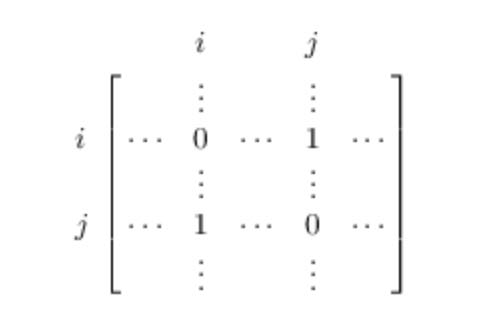
\includegraphics[width=0.5\textwidth]{ero1.png}
\end{figure}

			\item $i = a \times i$
			
			\IfFileExists{ero2.png}{}{\write18{wget https://cdn.mathpix.com/snip/images/w3ZfprTl-QheBb3U_I8ewNn9otmE_6E-7HOG5EPGqbg.original.fullsize.png -O ero2.png}}
\begin{figure}[H]
\centering
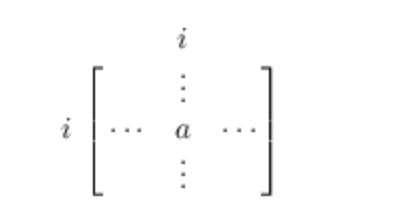
\includegraphics[width=0.5\textwidth]{ero2.png}
\end{figure}
			
			\item $ i = i + aj$
			
			\IfFileExists{ero3.png}{}{\write18{wget  https://cdn.mathpix.com/snip/images/fzYJHq5aPf7y9Hio2iAdrAaaOV8gnyyG-5ORD7kARiE.original.fullsize.png -O ero3.png}}
\begin{figure}[H]
\centering
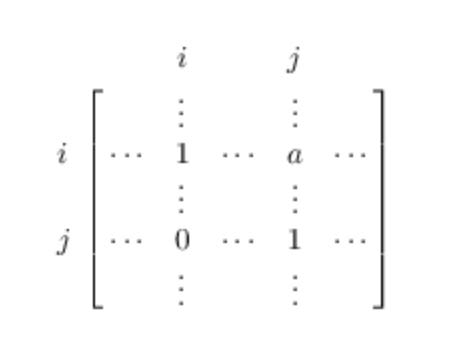
\includegraphics[width=0.5\textwidth]{ero3.png}
\end{figure}

\end{enumerate}
		
		\par{Key Insight: Each RO on $A$ is equivalent to left-multiplying $A$ by the equivalent elementary matrix}
	      	
		
		\extra{Computation}{
		Express an invertible matrix as a product of elementary matrices
		\begin{enumerate}
			\item Write down the augmented matrix $A | I$
			\item Apply subsequent  EROs , until $ I | A^{-1}$ . Taking note of each ERO
			\item Premultiply each ERO by $A$ in the order applied ,  $E_{n} \dots E_{1}A = I$
			\item Simplify , $(E_{n} \dots E_{1})^{-1}A = (E_{n} \dots E_{1})^{-1} \iff A = E_{n}^{-1} \dots E_{1}^{-1}$
		\end{enumerate}
		}
		 
		
		\subsection{Spaces}
		
	      	\defn{Space}{}
	      	
	      	\par{Informally, a space is a set of vectors composed of all possible linear combinations of all vector(s) in that space. In other words, I can choose one or more vectors in that space and I can add and multiply them and never leave that space. Crucially, this must include a way to get back to the origin, hence the $0$ vector must be part of every space.}
	      	
	      	\rem{All objects within a space must go through the origin (e.g. line in $\mathbb{R}^{2}$, plane in $\mathbb{R}^{3}$)}
	      	
	      	\par{We call a space entirely contained within another space $S$, a \ita{subspace} of $S$. So a subspace , $S_{b}$ of $S$ , is a space within which all the vector operations on $S$ are defined on $S_{b}$ but where usually some other conditions have to be satisfied, so that performing those operations on the members of $S_{b}$ imply never leaving $S_{b}$ and $S$ }
	      	\rem{A common example of subsets which are not subspaces are those which do not go through the origin of $S$. Given that they are defined for all operations on $S_{b}$ , however scalar multiplication by $0$ is not defined}
	      	
	      	\par{Note that for a matrix $A_{m \times n}$ , its columns linear combinations form a subspace of $R^{m}$. In order to picture why, think of $R^{3}$. Each vector represents \ita{``one part of the 3D''} , but by themselves they can't represent a space. Geometrically they represent 3 finite individual line segments. However, by including all possible linear combinations we \ita{fill in} the space between them, effectively representing all possible planes within $R^{3}$ , or all possible planes which satisfy some part of $R^{3}$ given some condition (e.g. positive numbers) }
	      	
	      	\defn{Column Space}{}
	      	
	      	\par{Note then, that the above means that we are essentially asking whether $A\vc{x} = \vc{b}$ is within $R^{m}$, and if so then for what $\vc{x}$. Now, given that the column space \ita{by definition} contain all possible combinations, then it contains all possible $A\vc{x}$; Hence,  $A\vc{x} = \vc{b} \iff \vc{b} \in C(A)$ }
	      	
	      	\example{\cite{mit:null}}
	      	
	      	\par{A specially useful corollary which follows from above, is that one can find all possible solutions for an homogenous system if we set $\vc{b} = \vc{0}.$}
	      	
	      	\prop{}{The set of solutions of an homogenous system $A$ is the null space of the augmented matrix $[A|\vc{0}]$}
	      	
	      	\proofs{It follows directly from above, and from the definition of an homogenous system}
	      	\newpage

%%%%%%%%%%%%%%%%%%%%%%%%%%%%%%%%%%%%% WEEK4	  %%%%%%%%%%%%%%%%%%%%%%%%
	      	\section{Basis, Dimensions, Rank}
	      	
		\rem{A basis is never unique}
	      	
	      	 RANK COMPUTATION : Once in row echelon form, the rank is clearly the same for both row rank and column rank, and equals the number of pivots (or basic columns) and also the number of non-zero rows
		
		\par{It is sometimes convenient to find a basis for the row space from among the rows of the original matrix instead . Since row operations can affect linear dependence relations of the row vectors, $A^{T}$ can be used instead. If a column of $A^{T}$ forms a basis of the column space of $A^{T}$ (i.e if there's a leading one), then it indicates that the corresponding rows in $A$ form a basis of the row space of $A$, before any EROs are applied. This is because $col(A) = row(A^{T})$  }
	      	
	      	%\todo*{Colum Space example MIT lecture}
	      	%\todo*{Bibtex: \url{http://sites.millersville.edu/bikenaga/linear-algebra/inverse/inverse.html} ; \url{https://ocw.mit.edu/courses/mathematics/18-06-linear-algebra-spring-2010/video-lectures/lecture-6-column-space-and-nullspace/} ; \url{https://math.stackexchange.com/questions/56201/how-to-tell-if-a-set-of-vectors-spans-a-space}}
		
		
	      	%\todos
		
	      	%\nocite{*}
	      	%\printbibliography
	      	
\end{document}